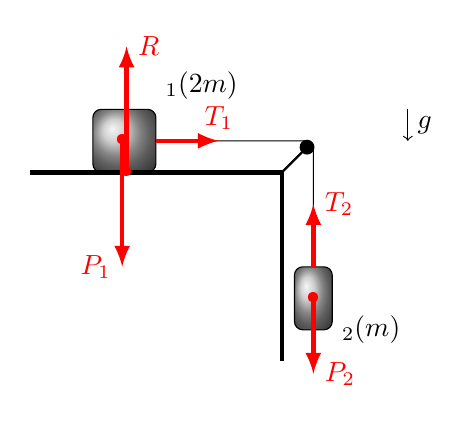
\begin{tikzpicture} [scale=.8]%,font=\footnotesize] 
		% blocs
		\draw[ball color=lightgray,rounded corners=3pt] (-3,0) rectangle (-2,1) node[above right]{$\ptB_1 (2m)$}; 
		\draw[ball color=lightgray,rounded corners=3pt](0.2,-1.5)rectangle (0.8,-2.5)node[right]{$\ptB_2 (m)$}; 
		% support	
		\draw[ultra thick] (-4,0)-|(0,-3);
		% fil
		\draw[rounded corners=3pt] (-2,0.5) --(0.5,0.5)--++(0,-2) ; 	
		\draw[thick,fill] (0,0)--(0.4,0.4) circle(0.1); 
		% forces
		\draw[-latex, ultra thick,red](-2,.5)--+(1,0)node[above]{$\vv{T_1}$};
		\draw[-latex, ultra thick,red](.5,-1.5)--+(0,1)node[right]{$\vv{T_2}$};
		\draw[-latex, ultra thick,red](.5,-2)node{•}--+(0,-1.2)node[right]{$\vv{P_2}$};
		\draw[-latex, ultra thick,red,shift={(-1pt,0)}](-2.5,.5)node{•}--+(0,-2)node[left]{$\vv{P_1}$};
		\draw[-latex, ultra thick,red,shift={(1pt,0)}](-2.5,0)node{•}--+(0,2)node[right]{$\vv{R}$};	
		\draw[->,shift={(2,1)}] (0,0)--+(0,-0.5) node[midway,right]{$\vv{g}$};	
\end{tikzpicture}